
% TODO
% Goal+contributie in abstract (ook real-time constaint)
% Contributies einde van intro

% Vragen aan Erwin
%        - Algemeen: Ik zie vaak dat je een uitleg verwacht eerder dan wanneer ik het zelf zou verwachten. In de intro/related work geef ik alleen een overview, later defineer je echt alles. Als je dit niet doet wordt je intro zo lang en technisch, wat mogelijk lezers afschrikt.
% Intro:
%        - Eerste alinea verwoord, beter zo?
%        - "is well suited for real-time transcrption". De intro lijkt mij niet de plek om hier heel uitgebreid op in te gaan, dat gebeurd ook later in de paper.
%        - "Most papers do not publish their source code, which makes building upon other's work difficult". Als een paper de methode "mathematically defined", betekend het niet dat het mogelijk is om erop verder te bouwen. De meeste papers zijn erg slordig in hun wiskunde noteren en het is ook niet altijd voor iedereen te begrijpen. Vaak missen er ook belangrijke details om iets net zo goed na te maken. Maar dit zijn slechts mogelijke verklaringen, in het veld zie ik verrassend weinig mensen op elkaars werk doorbouwen en zie ik veel mensen het wiel opnieuw uitvinden, wat duidelijk een probleem aantoont.
%        - Wat bedoel je precies met de real-time in quotes?
% Related work:
%        - Zijn de statements aan het einde van "related work" beter zo? (minder ad hoc)?
% Preliminaries:
%        - "You describe it as if this always happens...". Dat is toch ook zo?
% 5.1: Programming choises in different section. Dan wordt dit een sectie van 2 regels. Is het dan niet handiger om het gewoon in de corresponderende subsectie van implentation te laten?

% Antwoorden op jouw vragen
%       "experiment if Fourier methods are feasible for real-time transcription"->"is dat niet al gedaan?". Nee, in ieder geval niet praktisch. Er zijn een hoop papers die er een mening over hebben, maar weinig echte polyphone AMT systemen.
%       "accurately interpolate"->"estimate?". We interpoleren echt tussen 3 frequency bins. De hoogte van de frequency bins zouden eerder estimates zijn.
%       "such as the constant Q tranform"->"Why not use this tranform then?". Dit beschrijf ik als het goed is in de paper, maar omdat de Fourier erg snel is en veel onderzocht is.
%       "can be detected using another Fourier transform"->"what do you mean? explain". Voor nu iets anders verwoord, maar is het idee niet dat als je daar meer over wilt weten, je naar de referentie gaat?
%       Er missen bij veel referenties journal verwijzingen. In deze gevallen is het niet te vinden. Ik weet hier ook niet of het gewoon direct door een universiteit is uitgebracht of wat.
% 6.1: "Can the recordings not be improved?". Dat is een beetje vals spelen. Als ik dat zou doen, zou ik gewoon net zo lang kunnen blijven recorden totdat ik op zo'n manier speel dat het systeem 100% haalt.

\documentclass[10pt,twocolumn]{article}

% \frenchspacing
% \setlength\parindent{0pt}

\usepackage[english]{babel}
\usepackage[stretch=10, shrink=10]{microtype}
\usepackage[a4paper, total={6.5in, 9in}]{geometry}
\usepackage{graphicx}
\usepackage{caption}
\usepackage{subcaption}
\usepackage{amsmath}
\usepackage{multirow}
\usepackage{xcolor}
\usepackage{hyperref}
\usepackage{float}
\usepackage[linesnumbered,lined,commentsnumbered]{algorithm2e}

% Better vspace in enumerate/itemize
\usepackage{enumitem}
\setlist{noitemsep,topsep=0pt,parsep=0pt,partopsep=0pt}

% \setlength{\columnsep}{8mm}

\title{\textbf{Real-time guitar transcription using\\Fourier transform based methods}\\A pitch estimation framework and overtone sieve algorithm}
\author{Luc de Jonckheere}
% \date{}

\begin{document}
\selectlanguage{english}

\maketitle
%\tableofcontents


\section*{Abstract}
In this paper, we explore real-time transcription of an electric guitar signal. We focus on Fourier transform based methods, as this transform can be performed very fast. Using the obtained frequency domain, we select significant peaks using a Gaussian envelope. These peaks contain many overtones, which are filtered using our overtone sieve algorithm.

We will develop a basis for monophonic transcription and a proof-of-concept algorithm for polyphonic transcription. The goal of this paper is to give an overview of the problems when trying to solve this problem and to provide an implementation in which different methods for peak picking and overtone sieving can be tested.
% In the field of automatic music transcription (AMT), data driven methods such as artificial intelligence and machine learning are becoming more popular by the year. This is especially true for multi-pitch estimation (also known as multiple $f_0$ estimation). Even though the results are getting better every year, little understanding of the problem is gained. The few papers which use mathematical models to solve this problem, do not publish their code which makes it difficult to build upon.

% In this paper, we will present an extensible pitch estimation system along with a harmonic sieve algorithm which can perform basic multi-pitch estimation. This system can be used as basis for further research of the individual components.


% benadrukken dat er weinig nieuws is, maar combinatie is van bestaande dingen
\section{Introduction}
% Automatic Music Transcription (AMT) is a field of study which tries to automatically convert acoustic recordings into some form of (digital) music notation~\cite{survey1}. This task can be divided into two subproblems: pitch estimation and onset detection~\cite{survey2}. Instead of trying to convert a song into music notation, this paper will focus on translating a guitar signal into a set of played notes in real-time. This problem is very similar to AMT, as both require pitch estimation and onset/offset detection, however, we also have take latency into account.
Automatic Music Transcription (AMT) is a field of study which tries to automatically convert acoustic recordings into some form of (digital) music notation~\cite{survey1}. In this paper, we will focus on translating a guitar signal into a set of played notes in real-time. This task is similar to AMT, because both have to solve the problem of pitch estimation and onset/offset detection~\cite{survey2}. Because we try to solve the problem in real-time, we have some extra limitations. We must process the data fast enough such that no significant latency is introduced. Furthermore, we must process the data at least as fast as it is generated, otherwise latency would increase over time. Lastly, we cannot look-ahead, as can be done when transcribing pre-recorded songs.

Single pitch estimation can be accurately performed using Fourier transform based methods~\cite{mono}. Multi pitch estimation is much harder as harmonic overtones are difficult to differentiate from the fundamental frequency~\cite{oud}. As the Fourier transform can be performed consistently and efficiently on common hardware~\cite{fourierspeed}, it is well suited for real-time transcription.  % Because of this, most recent methods use machine learning or artificial intelligence. These methods are not well suited for real-time transcription. Also, little mathematical understanding of the problem is gained. Because of this, this paper will focus on mathematically solving this problem. Even if the methods researched in this paper might not outperform ML/AI solutions by themselves, they could be used to filter the input data for the ML/AI approaches. This might in turn improve the results of the AI/ML methods significantly.

Pitch estimation can be divided into a few subproblems. If a paper focuses on one of these subproblems, it also has to solve the other subproblems in order to test the system. Most papers do not publish their source code, which makes building upon other's work difficult. It also limits the research of the interaction between different solutions for the different subproblems. Because of this, we provide a framework which can be built upon, as the implementation of a subproblem can easily be interchanged with another. The code can be found at "\url{github.com/lucmans/dechord}".

The goal of this paper is to give a complete overview of the methods used to solve this problem. This is done by developing a program which can translate a guitar signal to a set of observed notes in real-time. We combine techniques spread over different papers into one project and provide an algorithm which can estimate a set of played notes using the set of observed notes. The code should be publicly available and easily extensible so others can optimize a subproblem without having to solve the other subproblems. Using our program, we can experiment if Fourier transform based methods are feasible for real-time transcription.

% Note that this paper is a preliminary paper for a possible master thesis. The focus is on building a prototype which can perform monophonic AMT and presenting a first draft of a polyphonic version. Using this information, we will estimate if the thesis project is feasible.
The focus of this paper is on building a prototype which can perform monophonic AMT and presenting a first draft of a polyphonic version. 


\section{Related work}
Spectral peak picking based AMT methods are often deemed infeasible for real-time AMT~\cite{hater}, due to the relatively low resolution in the low frequencies when using the Fourier transform~\cite{theoretisch}. This problem cannot be alleviated by zero-padding the Fourier transform input, as it does not add any information, it merely increases the resolution by interpolation~\cite{infomax}\cite{infomax2} and increases the computing time of the transform~\cite{boek}. However, using quadratic interpolation, we can very accurately interpolate peaks within Fourier frequency bins~\cite{interpol}. Also, other transforms such as the constant Q transform~\cite{cqt} which do provide more resolution in lower frequencies are getting more popular, which will allow us to differentiate two notes on a very small interval.

A big problem in polyphonic pitch estimation is the occurrence of overtones~\cite{oud}. As these overtones also have a periodic nature, they can be detected using another Fourier transform~\cite{double} on the obtained frequency domain. However, this periodicity also be detected with less overhead using note sets, which are explained in Section~\ref{sec:noteset_intro}. Notes which are at octave intervals have the same periodicity~\cite{octave}, which makes them difficult to distinguish. This is often referred to as the octave problem.

Another problem is choosing the real-time constraint for processing the input. Some papers claim 140 ms is sufficient~\cite{sloomboi}. This is however too long, considering it would be about a note difference when playing eight notes in 200 BPM. Furthermore, there always is a latency from the operating system due to how audio drivers work~\cite{os}.  % In practice, musicians often tweak their audio driver settings in order to gain 5 to 10 ms in latency, which makes the difference between being able to play faster pieces or not.

When focussing on transcribing a guitar, we can use physical limitations of the instrument to our advantage~\cite{physical}. However, by taking these limitation into consideration, the resulting program will be less versatile. For instance, these methods fail when the strings are tuned to different notes.


\section{Preliminaries}
In this paper, we use the Fourier transform to obtain a frequency domain representation of a signal. This transform takes a frame full of samples and produces a list of amplitudes corresponding to frequency bins. When performing the Fourier transform on a frame, spectral leakage is introduced~\cite{spectral}. This kind of noise is remedied by applying a window function to a frame. %How this is done is described in Section~\ref{sub:four}.

When playing a note on an instrument, multiple frequencies are produced. The most notable is the fundamental frequency. Every note corresponds to one fundamental frequency. Integer multiples of the fundamental frequency resonate and produce harmonic overtones~\cite{overtones}. They are called harmonic overtones, as they are exact integer multiples and do not produce destructive interference among each other. Every integer multiple resonates with the fundamental frequency, however, each subsequent overtone is of lower amplitude.  % For instance, the fundamental frequency of the $\text{A}_4$ is 440 Hz.

Generally, instruments do not produce perfect sine waves. The specific distortion of an instrument is called its timbre~\cite{timbre}. Even though the frequency components of these distortions are insignificant compared to the fundamental frequency and its overtones, it still results in extra noise in the signal. When strumming a note on the guitar, there is a strong attack. During this attack, the signal behaves chaotically and results in many fluctuating peaks in the frequency domain. This phenomenon is called a transient.

To specify in what octave a certain note lies, we use scientific note notation. This adds a subscript octave number to a note name. In scientific notation, we start from the note C. In other words, these notes are denoted in increasing pitch: $\text{C}_3$, $\text{A}_3$ and $\text{C}_4$. Note that $\text{A}_3$ is higher pitches than $\text{C}_3$, which is counter intuitive.

Most modern instruments use the twelve-tone equal temperament tuning system (12-TET). This tuning system divides an octave, which the distance between a frequency and its double, into twelve equal parts on the logarithmic scale. In other words, the ratio between two contiguous notes is $\sqrt[12]{2}$. The distance between two notes can further be divided on a logarithmic scale into 100 cents. The number of cents between two frequencies can be calculated as $1200 * \log_2(\frac{f_1}{f_2})$. 12-TET is tuned relative to a standard pitch. In modern music, we define the $\text{A}_4$ to be 440 Hz.


\section{Pitch estimation}
Automatic music transcription can be separated into two main problems; onset detection and pitch estimation~\cite{survey2}. In this paper, we will focus on pitch estimation. Onset detection is done implicitly, as we always output the set of played notes for the last analysed frame. If a note is added to the set of played notes, it can be considered as an onset. However, actual onset detection can improve the results of pitch estimation. For example, when an onset is detected, we can discard all samples from the transient that arises from this onset.

Pitch detection can be broken down into a few subproblems. First, a frequency domain representation of the signal is obtained (e.g. Fourier transform). Then, significant peaks have to be selected from the frequency domain. Based on the found peaks, we have to determine what notes were actually played on the instrument.

\subsection{Transform to frequency domain}
To estimate the frequency components of a frame, transforms are used. Most commonly, the Fourier transform is used as it is the most researched transform and much is known about it~\cite{survey2}. Its main downside is that the frequency bins are constant in size, where the distance between notes increases exponentially. Because of this, low notes are hard to discern in the frequency domain where high notes have more resolution than needed. Because of this, other transforms such as the constant Q transform (CQT) are getting more popular. Despite this, we will still use the Fourier transform as very efficient implementations exist for this transform. We need this efficiency to remain real-time.

%When using transforms, window functions have to by applied to the frames to prevent spectral leakage~\cite{window}. Furthermore, the actual peak locations can be accurately interpolated using (Lagrangian) quadratic interpolation~\cite{interpol}.% These concepts are further described in Section~\ref{sub:four} and Section~\ref{sub:peak} respectively.
When using the Fourier transform, a window function has to be applied to a frame to prevent spectral leakage~\cite{window}. In this paper, we use the Blackman-Nuttall window. Given a window with $N$ samples, the Blackman-Nuttall window $w(n)$ is defined as:\vspace{-1mm}
\begin{center}
    \hspace{-12mm} $w(n) = 0.3635819 - 0.4891775*\cos(\frac{2\pi n}{N})$ \\\vspace{+0.5mm}
    \hspace{+4mm} $+ 0.1365995 * \cos(\frac{4\pi n}{N}) - 0.0106411 * \cos(\frac{6\pi n}{N})$
\end{center}%\vspace{-2.5mm}
Then, with the signal $s(n)$ and the window $w(n)$, we can obtain the resulting windowed signal res$(n)$ using:
\begin{center}%\vspace{-2mm}
    $\text{res}(n) = s(n) * w(n)$
\end{center}
Figure~\ref{fig:spec} shows the effect of a window function on a frame graphically.
\begin{figure}[H]%\vspace{-2mm}
    \centering
    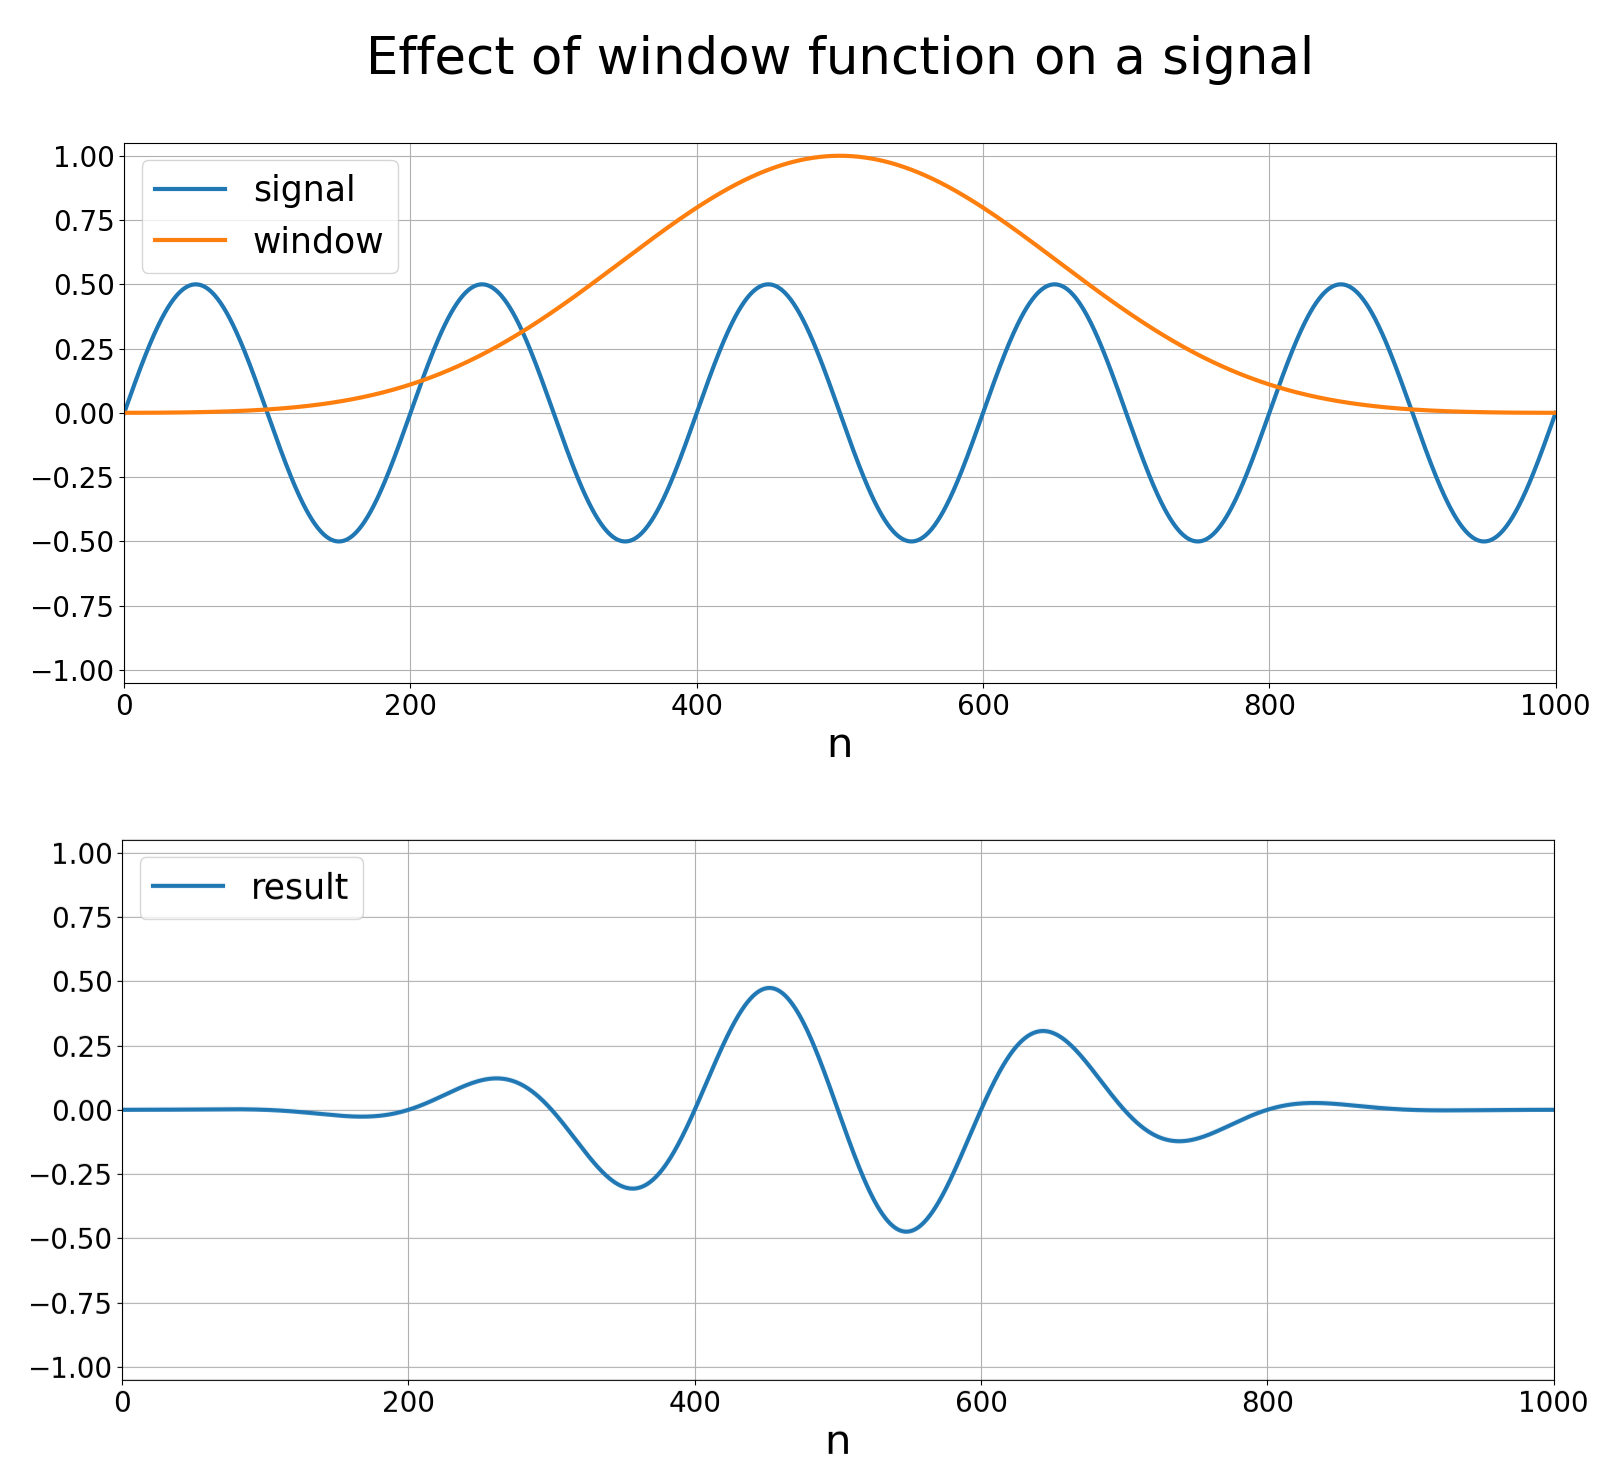
\includegraphics[width=\linewidth]{3.png} %0.85
    \caption{The effect of applying a window function to a signal}
    \label{fig:spec}
\end{figure}%\vspace{-4mm}
%In polyphonic signals, harmonic overtones of different notes can interfere, which will lead to inconsistent and oscillating peaks.  % TODO: Maybe make preliminary section about overtone dissonance

The output of a Fourier transform is a list of complex number. The norm of each complex number corresponds to the amplitude of a certain frequency bin. The size of these frequency bins $f_{\text{bin}}$ is determined by the sampling rate $f_{\text{SR}}$ of the signal (samples per second) and the number of samples in a frame SPF with the following relation:
\begin{center}
    $f_{\text{bin}} = \frac{f_{\text{SR}}}{\text{SPF}}$
\end{center}
Furthermore, the frame length $t_\text{frame}$ in seconds can be calculated as follows:
\begin{center}
    $t_{\text{frame}} = \frac{\text{SPF}}{f_{\text{SR}}}$
\end{center}
% Higher sampling rates give us more precision, but also requires more processing power. Also, widespread audio interfaces only offer sampling rates up to 192 kHz.

\subsection{Peak picking}
Peaks in the frequency domain correspond to predominant frequencies in the analysed frame. A peak is defined as a bin which has a higher amplitude than its left and right neighbour.

Not every peak is of interest. Some peaks are generated by noise in the signal. Many of these peaks can be filtered by requiring an arbitrary signal level to be considered a peak. This approach will however result in less sustain.

In order to determine if a peak is significant enough, we first calculate a Gaussian average envelope~\cite{gauss}. For every frequency bin, the Gaussian average is a weighted average of all frequency bins, where the weight is determined by the distance from the considered bin. Given a distance of $n$ bins, the weight is determined by the following Gaussian function:
\begin{center}
    $e^{-\pi(\frac{n}{\sigma})^2}$
\end{center}
Here, $\sigma$ can arbitrarily be chosen. Higher values for $\sigma$ make points close by weight more compared to distant points. By using the envelope, we effectively filter small local maxima close to large local maxima.

Every peak which surpass the envelope and is above the arbitrary signal level is deemed significant and used in the next step, the harmonic overtone sieve. We also provided a different variant of the peak picker where only the highest peak is selected for every lobe which surpasses the envelope and a variant which picks all peaks, disregarding the envelope. We also provided a peak picker which picks every peak, which is useful for development purposes.

\subsection{Harmonic overtone sieve}  \label{sec:noteset_intro}
Given the significant spectral peaks from the previous step, we can try to calculate what notes they represent. First, we get the actual location of a peak with a Fourier bin using quadratic interpolation~\cite{interpol}\cite{interpol2}. Here, we calculate a value $p \in [-\frac{1}{2}, \frac{1}{2}]$, which is the location of the actual peak relative to the found peak in number of Fourier bins. In order to calculate $p$, we need the height of our found peak ($y(0)$) and the height of the two neighbouring bins ($y(-1)$ and $y(1)$). As quadratic interpolation is more accurate in the dB (logarithmic) scale, we define:
\begin{center}%\vspace{-3mm}
    $\alpha = \log y(-1)$\\
    $\beta = \log y(0)$\\
    $\gamma = \log y(1)$
\end{center}%\vspace{-1mm}
Then, we can calculate $p$ as follows:
\begin{center}%\vspace{-1mm}
    $p = \frac{1}{2} \cdot \frac{\alpha - \gamma}{\alpha - 2\beta + \gamma}$
\end{center}%\vspace{-1mm}
Given $p$, we can also calculate the amplitude $a$ corresponding to the interpolated location:
\begin{center}
    $a = \beta - \frac{(\alpha - \gamma) * p}{4}$
\end{center}
Now, we can calculate the frequency of the peak $i$ by multiplying the Fourier bin size by $i + p$. Using the obtained frequencies and corresponding amplitudes, we construct note sets. A note contains all useful information about the peak for transcription. Other than the interpolated frequency and corresponding amplitude, we calculate the distance to the closest note in cents and we also store the scientific pitch notation. To calculate the distance between our interpolated frequency $f_i$ and the closest note, we first calculate the tuned frequency $f_t$:
\begin{center}
    $f_t = f_{\text{A}_4} * 2^{\text{round}(12 * \log_2(\frac{f_i}{f_{\text{A}_4}})) / 12}$  %exp2(round(12.0 * l2) / 12.0)
\end{center}
Then, we can calculate the distance $d$:
\begin{center}
    $d = 1200 * \log_2(\frac{f_i}{f_t})$
\end{center}
Given an array with all the note names (A, A\#, B, C, C\# etc.), we can calculate the index which contains the name of the note as follows:
\begin{center}
    $i = \text{round}(12 * \log_2(\frac{f_i}{f_{\text{A}_4}}) \mod 12)$
\end{center}
Here, we assume that "$-1 \mod 12 = 11$", which is not the case in all programming languages. To calculate the octave number, we first calculate the pitch of $\text{C}_1$:
\begin{center}
    $f_{\text{C}_1} = f_{\text{A}_4} * 2^{\frac{45}{12}}$
\end{center}
Using this, we can calculate the octave number $o$:
\begin{center}
    $o = \text{floor}(\log_2(\frac{f_i}{f_{\text{C}_1}}) + 1)$
\end{center}
Note that this equation fails if we calculate the octave number of a $C$ which is tuned too low ($f_i < f_t$). To remedy this, we can simply add a check if this is the case and increment the octave number accordingly.
%
% Usually, peaks do not exactly coincide with a note. In order to calculate the error in cents, we need the tuned frequency $f_t$ of the closest note to our observed frequency $f_o$. First, we have to calculate the number of semitones $n$ ($\sqrt[12]{2}$ steps) it is removed from a tuning note, such as the $\text{A}_4$:
% \begin{center}
%     $n = \text{round}(12 * \log_2(\frac{f_o}{f_{\text{A}_4}}))$
% \end{center}
% The decimal part of $n$ before rounding would be the amount of dissonance. By rounding this number, we find the closest note. Now, we can calculate the tuned frequency by doing the inverse of the previous calculation:
% \begin{center}\vspace{-3mm}
%     $f_t = f_{\text{A}_4} * 2^{\frac{n}{12}}$
% \end{center}
% Using this tuned frequency, we can calculate the error $e$ in cents as follows:
% \begin{center}
%     $e = 1200 * \log_2(\frac{f_o}{f_t})$
% \end{center}
% If the guitar is tuned and intonated correctly, we can set a threshold on the error of a detected note. Only notes within this threshold can be fundamental notes.

Unfortunately, a note set does not only contain fundamental frequencies, but also harmonic overtones. This is only a small problem in monophonic transcription, as there is only one fundamental frequency and its overtones. However, in the polyphonic case, it is difficult to determine which peaks are fundamentals and by extension know how many notes are played at the same time.

To determine if notes are fundamentals or overtones, we developed a "harmonic overtone sieve" algorithm. This algorithm iterates over all found peaks and checks if any higher pitched peak is a possible overtone of the considered peak. As the calculated frequency of a peak may not be accurate, we have to set a threshold on the error under which a peak is considered an overtone. Because the distance between notes increases with frequency, we cannot set a constant threshold of error in Hz. Therefore, we calculate the error in cents and choose a threshold for this error. This also allows for equal error tolerance above and below the note, which percentage based methods would not. Given the frequency of the considered peak $f_c$ and the possible overtone $f_o$, we can calculate the frequency of the closest harmonic overtone $f_h$:
\begin{center}
    $f_h = f_c * \text{round}(\frac{f_o}{f_c})$
\end{center}
Using the closest harmonic overtone frequency, we can calculate the error from our possible overtone in cents:
\begin{center}
    $e = 1200 * \log_2(\frac{f_o}{f_h})$
\end{center}
T

For every peak, we keep track of two variables. The first is the number of number of overtones we detected for every peak. The second is a boolean which indicates if a peak is a overtone of another peak. For monophonic note detection, we can assume that the peak with the most overtones is the fundamental frequency. For polyphonic note detection, we can assume that every peak which is not an overtone of another lower pitches peak is a fundamental. Another method for polyphonic note detection would be setting a threshold for the number of overtones a fundamental should have. This however gives inconsistent results, because when the same note is played louder, more overtones are detected. Furthermore, the number of overtones decreases while a note sustains.

A guitar has a limited range of fundamental tones which it can produce. Using this information, we can discard all peaks lower than the lowest fundamental of a guitar as noise and mark all peaks higher than the highest fundamental as overtones or noise. These ranges have to be configurable to accommodate different tunings or guitars with extra strings or frets.

Overtones are dissonant relative to our scale. The error of an overtone is calculated as the number of cents from the closest harmonic note. The errors are different for every overtone, but the series of errors is constant for every harmonic overtone series. In Table~\ref{tab:overseries}, we provided the errors of the first 6 overtones.
\begin{table}[H]\vspace{-3mm}
    \centering
    \begin{tabular}{rrcrr}
        $n$ & $f_{\text{overtone}}$ & closest note & $f_\text{note}$ & error \\
        \hline
        0 & 261.626  & $C_4$    & 261.626  &  - \\
        1 & 523.251  & $C_5$    & 523.251  &  0 \\
        2 & 784.877  & $G_5$    & 783.991  &  1.955 \\
        3 & 1046.502 & $C_6$    & 1046.502 &  0 \\
        4 & 1308.128 & $E_6$    & 1318.510 &  -13.686 \\
        5 & 1569.753 & $G_6$    & 1567.982 &  1.955 \\
        6 & 1831.379 & $A^\#_6$ & 1864.655 &  -31.174 \\
    \end{tabular}
    \caption{Example of overtone series and the errors compared to the closest note}
    \label{tab:overseries}
\end{table}\vspace{-3mm}
If only harmonic notes were played on a guitar, we could filter all notes with an error higher than an arbitrary threshold. However, as most guitars are not perfectly intonated and strings detune by pressing them down on a fret, this information has to be used with care. Correctly using this information is out of the scope of this paper.


\section{Implementation}  \label{sec:impl}
The program developed for this paper is written in C++ (11) and compiled with g++ (10.2.0). It uses SDL (2.0.14) for audio input/output and spectrum visualisation. FFTW (3.3.9) is used for efficient Fourier transforms. Its code can be found at "\url{github.com/lucmans/dechord}".
%
% There are many parameters which change the behaviour of the overall system. For this paper, we choose some values which seemed to perform well. The values can still be optimized for better results. All parameters can be found in \texttt{config.h} along with comments explaining them.

By default, the program assumes an $A_4$ of 440 Hz. Only 12 tone equal temperament (12-TET) tuning is currently supported. Our framework can be changed to other TET tunings, but non TET tuning is not easily supported.

An pseudo-code overview of the transcription process is given in Algorithm~\ref{alg:overview}. We first obtain a frame of samples from the audio driver. After applying a window function to it, we perform the Fourier transform on it. To get the amplitudes of every frequency bin, we have to calculate the norm of the output of the Fourier transform. We then calculate the Gaussian envelope of the frequency domain and find the location of these peaks. Using the peak locations, we can interpolate the actual frequency corresponding to each peak and build a set of notes from these peaks. Using our harmonic overtone sieve algorithm, we can perform monophonic or polyphonic transcription.
\input{overview.pc}

\subsection{Transform to frequency domain}  \label{sub:four}
As mentioned before, the resolution of the Fourier transform depends two parameters, the sampling rate and the number of samples in a frame. When using a higher sampling rate we increase the resolution of the Fourier transform. This also increases the computation power required to process one second of samples. We are limited to a sampling rate of 192 kHz, as this is the maximum for most audio interfaces and audio drivers. To allow guitarists to play mildly fast, we have to limit our frame length. If the frame size if too large, multiple separate notes may be included in one transform, which would make it seem like the notes were played at the same time. Moreover, frame sizes which are a power of two can be transformed more efficiently, which further restricts are frame size choice. For example, if we choose a frame size of $2^{14} = 16384$ samples at a sampling rate of 192 kHz, the frame length is 85.33 ms (11.72 frames per second). The corresponding Fourier bin size is 11.72 Hz. At first glance, such a large bin size seems like a big problem, as the smallest interval that can be played on a guitar (G\#\textsubscript{2}-A\textsubscript{2}) is about 6 Hz. However, the overtones of these notes will have more Hz between them, which makes to possible to differentiate the two notes.% Also, as discussed in Section~\ref{sec:future}, we might be able to increase the frame size without reducing our frame rate too much.

Before applying the transform, a window function is applied to minimize the artifacts produced by the transform. The following windows are also provided: Hamming window, Hann window, Blackman window, Nuttall window, Blackman-Harris window, Blackman-Nuttall window, Flat top window. Other window functions can easily be added.

Because our input data is purely real, we know the output of the Fourier transform will be symmetric. For this reason, we can omit calculation half of the output. This results in an almost two times speed-up~\cite{twotimes}.

\subsection{Peak picking} \label{sub:peak}
Three different peak picking algorithms have been implemented. The main algorithm is based on the Gaussian envelope. First, the relevant points on the Gaussian function are calculated and stored in an array. Normally, at least as many values have to be precomputed as there are frequency bins. However, because values further in the tail are close to zero, we can omit calculating these values and subsequently skip calculation involving them in the Gaussian average, which serves as a slight optimization. Algorithm~\ref{alg:gauss} shows how the values on the Gaussian function are computed given a \texttt{kernel\_width}, which is the number of values we precompute.
\input{gauss.pc}

Using our previously computed values, we can calculate the Gaussian average envelope as shown in Algorithm~\ref{alg:env}. The envelope is calculated for every Fourier bin $i$ by calculating the weighted average of \texttt{kernel\_width} bins around $i$. As mentioned before, higher values of $\sigma$ result in points closer to $i$ to be weighted higher. In line 7, we use the \texttt{min} and \texttt{max} function to prevent array accesses outside of array bounds. Using this envelope, we can select all significant peaks as shown in Algorithm~\ref{alg:peak}. By commenting line 4, we obtain the algorithm which selects all peaks. Line 5 checks if a peak is loud enough to be considered a peak, which prevents finding peaks in noise.

The other method based on the Gaussian average envelope only select one peak every time a lobe surpasses the envelope. A possible implementation is given in Algorithm~\ref{alg:peak2}. Here, we keep track track of the highest peak found so far. Every time the amplitude of a bin dips below the envelope, we select the highest found peak and reset the currently highest found peak. This results in always picking the highest peak from a single lobe which surpasses the envelope. We split the if statement on line 7 into two check to prevent an invalid array access when \texttt{highest} is -1.
\input{env.pc}
% \vfill
\input{peak.pc}
% \vfill
\input{peak2.pc}

\subsection{Harmonic overtone sieve}  \label{sub:impnoteset}
An overview of the monophonic is given in Algorithm~\ref{alg:mono}. Here, we iterate over all found peaks and check if every higher peak can be an overtone of the considered peak. After counting the number of overtones for every peak, we can pick the peak with the most overtones.
\input{mono.pc}

Polyphonic note detection can use an algorithm similar to the monophonic algorithm. As the number of played notes is unknown in the polyphonic case, we have to determine if a note is a fundamental or overtone. As mentioned before, we cannot just set a threshold for the number of overtones a fundamental should have. To solve this problem, we present a harmonic overtone sieve algorithm. A pseudo-code implementation of this algorithm is shown in Algorithm~\ref{alg:poly}. Instead of directly looking for fundamentals, we try to sieve away all harmonics until we are left with fundamentals. We start at the lowest peak end mark all its possible overtones. If there are still unmarked peaks left, they are likely from another note and we sieve its overtones away. We can repeat this process until no more peaks can be sieved. Lastly, we can remove all peaks which are outside of the frequency range of a guitar. If two peaks are not distinguishable in the root notes but are distinguishable in the overtones, this algorithm will report the first distinguishable overtone as the root note. It is possible to calculate what the root note should have been, but that is outside the scope of this paper and will be further discussed in Section~\ref{sec:future}.
\input{poly.pc}

\subsection{Latency}
As stated before, our goal is to perform the transcription in real-time. We choose a constraint of 6 ms. Most musicians work with a driver latency of 9 to 11 ms. On a good computer, this latency can be reduced to 3-5 ms. We will use these 6 ms of latency difference to perform our calculations in. Note that when playing more notes per second, latency becomes more of a problem. On slower pieces, we can get away with much larger latencies. In order to test the impact of extra latency for yourself, we developed a tool which plays back the incoming audio signal with a user specifiable delay. This tool can be found under the "latency" branch in our GitHub repository. Note that this tool adds a latency on top of the audio driver latency like our program would. The total latency is much larger than the displayed latency.

The latency of our system results from two different latencies, the time to fill a frame with samples and the frame processing time. Because our algorithm works on a "per frame" basis instead of a "per sample" basis, we have to wait until the audio driver has fetched enough samples for us to fill a frame. The time it takes to start analysing a frame after receiving the first sample of this frame can be calculated by dividing the number of samples per frame by the sample rate. This is equal to the length of a frame. In practical terms, it is the maximum latency on detecting a newly played note. The average latency is obtained by dividing this number by two.

We use a frame size of 16384 samples and a sample rate of 192 kHz, which equates to a frame length of 85.3 ms. This is well over our real-time constraint. Unfortunately, we cannot change this value too much. The sample rate is already at the maximum of most audio interfaces. We also cannot lower the number of samples per frame while using the Fourier transform, as it would further reduce the frequency resolution. However, as will be explained in Section~\ref{sec:future}, this might not be a problem, as we can reduce this latency by using partially overlapping frames.

We can control the second kind of latency by optimizing our algorithms. In Section~\ref{sec:exp}, we will measure the processing time of the different algorithms.


\section{Experiments}  \label{sec:exp}
We will perform several experiments to test the performance of various aspects of our system. During development, an electric guitar with active EMG humbucker pickups was used. To convert the analog signal to a sampled digital signal, a Behringer UMC404HD was used. This audio interface has a dynamic range of 100 dB. As is the case for most audio interfaces, this is much less than the dynamic range of a sample (144 dB for 24 bit integer). We opted not to amplify the signal in software, as it will distort it; especially if not done carefully. The tests were performed on an AMD 3700X CPU.
%
% Often used datasets for evaluating pitch estimation focus on different goals than this paper. For instance, they focus on transcribing multiple instruments at once or having instrument invariance. They also do not focus on real-time transcription, which makes the problem much harder. However, in order to present some comparative measure, we will use the Mirex dataset for "Multiple Fundamental Frequency Estimation \& Tracking"~\cite{data}. TODO (when I receive it): Short description of dataset.

We constructed our own dataset to evaluate the performance. Our dataset consists of scales and intervals played on a guitar. Scales allow us to measure the monophonic performance. As scales are easy to play, multiple recordings should have the same results. This allows us to isolate and measure other variables, such as the effect of tempo or playing the scale higher/lower. Recordings of different intervals allow us to measure the polyphonic performance. By measuring all two note intervals, we can identify any problems with specific intervals. As the distance in frequency in an interval increases when the same interval is played at higher notes, we record the intervals at multiple root notes.% We will also measure the performance on the four basic triads: the major triad, minor triad, augmented triad and diminished triad.

Note that when repeating our experiments, your results may vary slightly. This is because the results of the Fourier transform from FFTW are not consistent~\cite{fftw}. This is especially noticeable in inconsistent latencies.

TODO: List of parameters!
% One algorithm picks all peaks which are above this average and the other only picks the highest peak for each spectral lobe above this average. Only picking the highest peak seemed to restrictive in testing, however, it is better resilient against noise and may be used with more careful parameter optimisation.

\subsection{Monophonic performance: scales}
To test the monophonic performance of our system, we first measure the performance of scales at different pitch ranges. The scales are played at a speed of two notes per second. This equates to playing fourth notes on 120 BPM. We play the scales at a relatively slow speed, such that this cannot become a limiting factor. The slower speed also helps to see if mistakes are the result of transients, as these mistakes should vanish as the note persists. We only play the C major scale, but change the starting note (mode). We play the full vertical scale from this starting note~\cite{scale}. Each position has 17 notes, except for $\text{F}_2$, which has 18 notes. In Table~\ref{tab:monperf}, we summarize the results of the experiment. We denote the different starting positions as $n_\text{start}$. For every starting position, we denote the accuracy ($a$), the accuracy without transient errors ($a_\text{trans}$), the accuracy without octave errors $a_\text{oct}$ and the adjusted accuracy without both of these errors ($a_\text{adj}$). The accuracy is calculated by dividing the number of correctly determined frames by the total number of frames with notes. The only frames without notes are positioned at the start and end of a file. We omitted these frames from the results, as they are always correctly determined to be empty frames. Erroneous notes due to transients usually have a lower amplitude where octave errors usually have a higher amplitude compared the amplitude of the base note. This allows is to distinguish between them. This information cannot be used to detect transients in real-time, as we compare the amplitude of the erroneous note to amplitude of the correct note in the following frames.
\begin{table}[H]\vspace{-3mm}
    \centering
    \begin{tabular}{r|rrrr}
        $n_\text{start}$ & $a$ & $a_\text{trans}$ & $a_\text{oct}$ & $a_\text{adj}$ \\
        \hline
        $\text{E}_2$ & 91.4\% & 95.2\% & 96.2\% & 100\% \\
        $\text{F}_2$ & 92.3\% & 96.2\% & 96.2\% & 100\% \\
        $\text{G}_2$ & 92.0\% & 95.0\% & 97.0\% & 100\% \\
        $\text{A}_2$ & 93.0\% & 94.0\% & 99.0\% & 100\% \\
        $\text{B}_2$ & 92.8\% & 96.9\% & 95.9\% & 100\% \\
        $\text{C}_3$ & 92.8\% & 92.8\% & 100\%  & 100\% \\
        $\text{D}_3$ & 96.0\% & 98.0\% & 98.0\% & 100\% \\
        $\text{E}_3$ & 96.7\% & 96.7\% & 100\%  & 100\%
    \end{tabular}
    \caption{Accuracy of monophonic $f_0$ estimation on C major scale at two notes per second for different starting positions. $a_\text{trans}$ is the accuracy without transient errors and $a_\text{oct}$ is without octave errors. $a_\text{adj}$ is the accuracy without both of these errors.}
    \label{tab:monperf}
\end{table}\vspace{-3mm}
We can see that the transient errors occur about 96\% of the time. There are two outliers at $\text{C}_3$ and $\text{D}_3$, which are the cause of inconsistent quality in the recording of the scales. This shows us that the guitarist has to play carefully for the best results. Furthermore, we noticed that the first played note almost always has a transient error. This could be because we start playing from a silent signal instead of changing from a previous note. Also, the transient errors show up more often between lower frequency notes. Almost all octave errors are at note changes, so better transient filtering will also solve these cases. Other than these errors, the system seems to work perfectly.

\subsection{Polyphonic performance: intervals}
To test the polyphonic performance of our system, we let it determine the played notes in an interval. We play every interval within an octave to test if there are any problems with separating the notes in specific intervals. For instance, some interference may cause oscillating peaks in the frequency domain. Again, we try all the intervals at different root notes, as the pitch of the root note may make a big difference in performance. As we mentioned before, when two peaks are too close together, we cannot distinguish them. Often, the second note is distinguished an octave higher. We set the overtone error threshold to 10 cents. This is a relatively small value, but this allows us to see small problems in our algorithms better. Furthermore, as shown in Table~\ref{tab:overseries}, we should not use a constant value, but use a different value for every $n$-th overtone. In Tables~\ref{tab:polperf1}--\ref{tab:polperf3} is a summary of the results. Here, we list the number of semitones $n$ between the two notes in an interval, if both notes were correctly found. If not, we denote if the second note was detected an octave higher. This often happens, because we cannot distinguish two notes in small intervals at low pitches. The last column shows if there were other notes reported which were not transients.

In the tables, we can see that the algorithm performs well on higher pitched intervals. On medium pitched intervals, the small intervals become more of a problem, but most intervals are detected correctly. Transients are however visible for longer in the small intervals. Big problems arise when we look at the lower pitched intervals. There is much noise in the results and many slightly inharmonic overtones are reported. These could be filtered out by increasing the overtone error threshold, but that does not solve the overtones being inharmonic. The inharmonic overtones are less of a problem for larger intervals.
%
% We also look at the percentage of overtones that is filtered throughout a recording of an interval.
% As the harmonic overtone sieve algorithm is only a proof of concept, absolute performance measurements will yield bad results. By measuring the performance relative to having no filtering, we can show the effectiveness of our algorithm. This is done by measuring the percentage of overtones that is filtered throughout a recording of an interval. TODO: See Figure~\ref{fig:relative} for some examples of 
%
% Lastly, we will measure the performance on the four main triads: the major triad, minor triad, augmented triad and diminished triad. TODO: Experiment
\begin{table}[H]%\vspace{-2mm}
    \centering
    \begin{tabular}{r|lll}
        $n$ & both & octave & other \\
        \hline
        1  & false & true & 1-3 slightly inharmonic overtones \\
        2  & false & false & - \\
        3  & false & true & $\text{C}_4$ and $\text{G}_4$ (+ random at start) \\
        4  & true & - & Sometimes octave instead\\ &&& and 1-2 inharmonics at start \\
        5  & true & - & 1 slightly inharmonic overtone \\
        6  & true & - & 1-3 slightly inharmonic overtones \\
        7  & true & - & no \\
        8  & true & - & no \\
        9  & true & - & occasional inharmonic overtone \\
        10 & true & - & 1-2 slightly inharmonic overtones \\
        11 & true & - & 1-2 slightly inharmonic overtones
    \end{tabular}
    \caption{Performance of distinguishing notes in an interval with root note $\text{A}_2$. Given an $n$ semitone interval, we list if we find both notes and if not, if one of the notes was found an octave higher. We also list the other reported notes.}
    \label{tab:polperf1}
\end{table}
\vspace{-3mm}
\begin{table}[H]
    \centering
    \begin{tabular}{r|lll}
        $n$ & both & octave & other \\
        \hline
        1  & false & true & about 4 slightly inharmonic overtones \\
        2  & false & true & about 4 slightly inharmonic overtones \\
        3  & true & - & $\text{C\#}_6$ or $\text{E}_6$ in first few frames \\
        4  & true & - & no \\
        5  & true & - & no \\
        6  & true & - & no \\
        7  & true & - & $\text{E}_4$ often filtered \\
        8  & true & - & random note 3 times \\
        9  & true & - & no \\
        10 & true & - & no \\
        11 & true & - & no
    \end{tabular}
    \caption{Performance of distinguishing notes in an interval with root note $\text{A}_3$.}
    \label{tab:polperf2}
\end{table}
\vspace{-3mm}
\begin{table}[H]
    \centering
    \begin{tabular}{r|lll}
        $n$ & both & octave & other \\
        \hline
        1  & false & true & occasional $\text{E}_6$ \\
        2  & true & - & no \\
        3  & true & - & no \\
        4  & true & - & no \\
        5  & true & - & no \\
        6  & true & - & no \\
        7  & true & - & no \\
        8  & true & - & no \\
        9  & true & - & no \\
        10 & true & - & no \\
        11 & true & - & no
    \end{tabular}
    \caption{Performance of distinguishing notes in an interval with root note $\text{A}_4$.}
    \label{tab:polperf3}
\end{table}%\vspace{-3mm}

\subsection{Latency}  \label{sub:algspeed}
The processing time of our system is very important, as it will directly impact the latency. We will only measure the time between receiving a frame from the audio driver until the answer is computed, as the time spent waiting on enough samples is fully determined by the number of samples in a frame and the sampling rate. The total processing time and the processing time of the individual steps and the total system can be seen in Figure~\ref{fig:snel}. Here, we only measure the latency on frames which contain peaks.

The total latency is never higher than 360 microseconds. Given that a frame is 85 milliseconds, we are at least 235 times real-time. This is well within out real-time constraint if we disregard the latency to fill a frame. Surprisingly, the peak picking algorithm is more computationally intensive than the transform. Most of the time, the latency is on the lower end of the distribution. The outliers are mostly a result of transients. During transients, there are a lot more peaks to process, which slows down the different algorithms. This is especially the case for polyphonic transcription, as we have to take all the peaks into account. In the polyphonic dataset, transients contain more peaks as multiple strings are strummed. This results in a second lobe in the mid segment of the latency distribution.
\begin{figure}[t]%\vspace{-2mm}
    \centering
    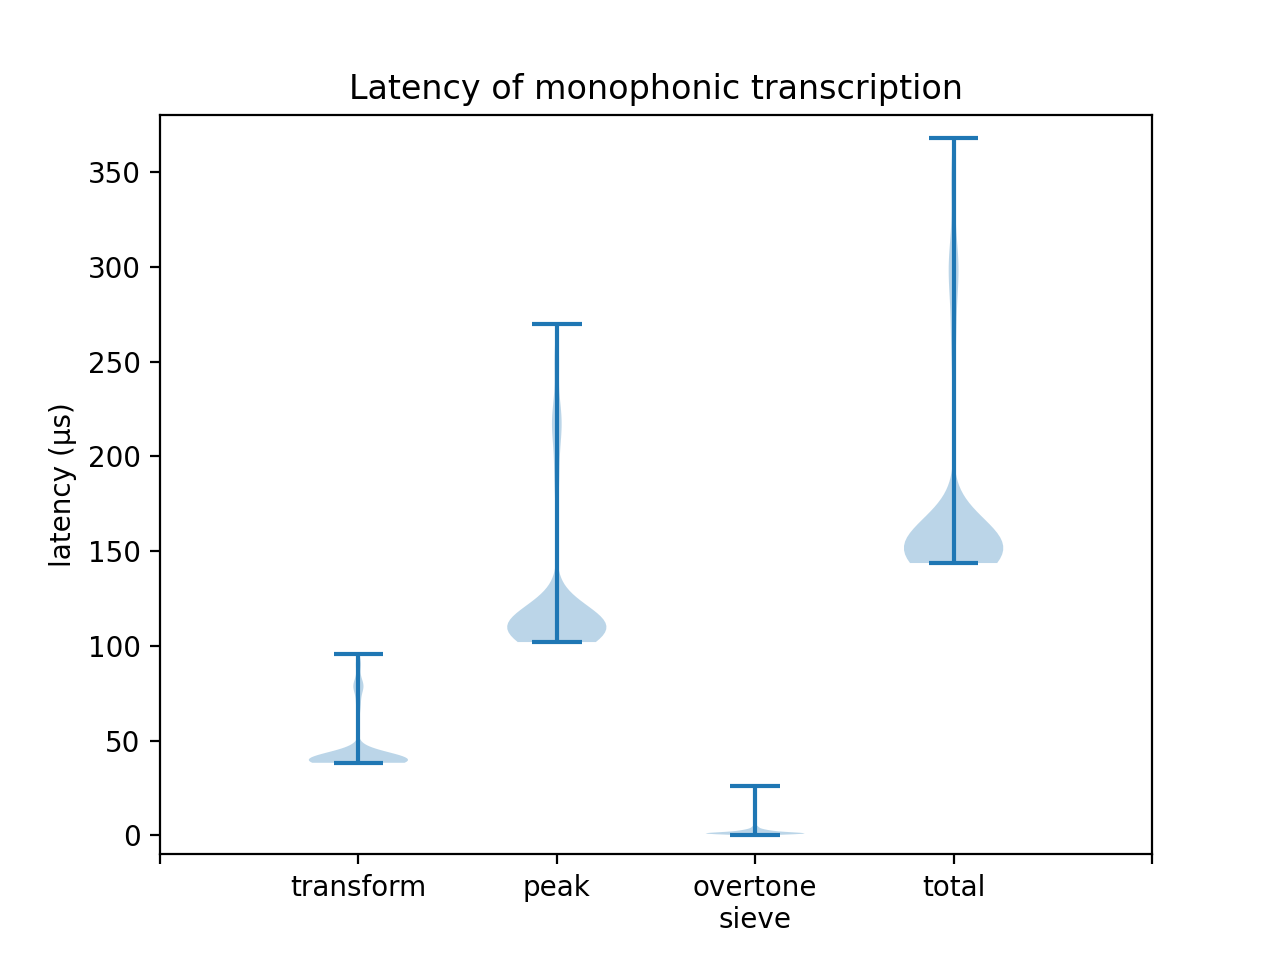
\includegraphics[width=\linewidth]{1.png}\vspace{+6mm} %0.85
    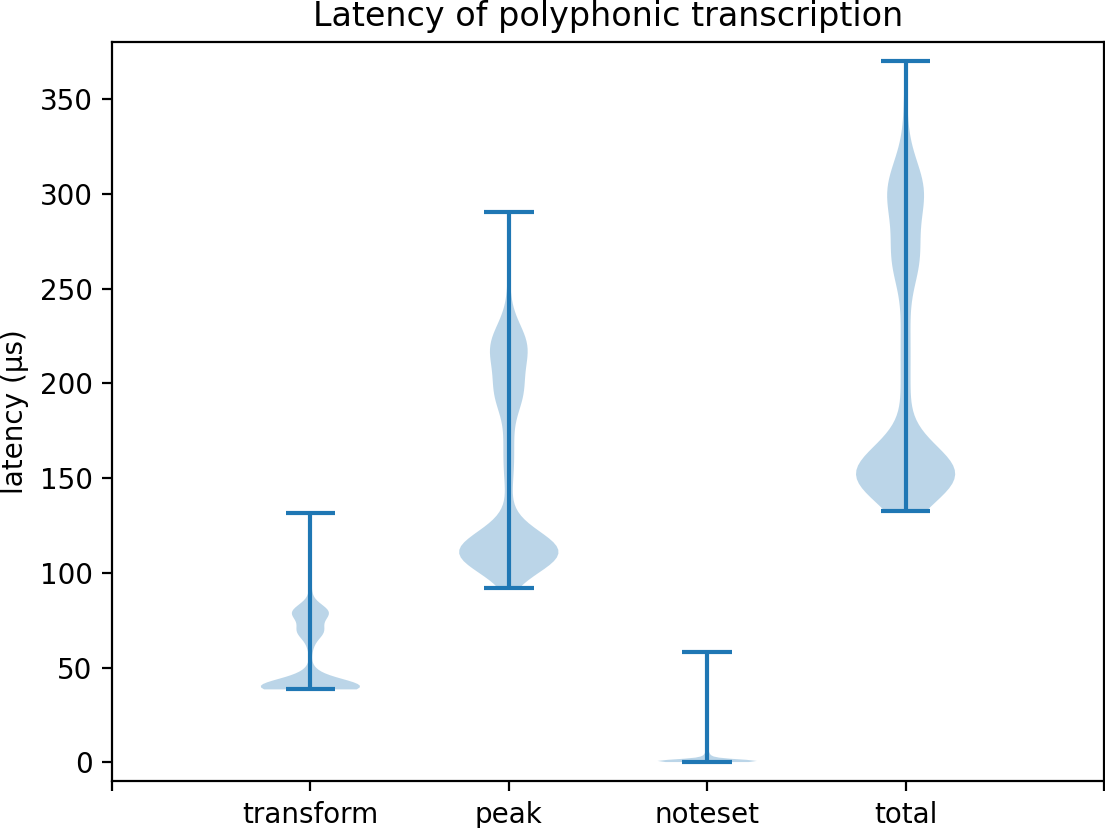
\includegraphics[width=\linewidth]{2.png} %0.85
    \caption{Processing time of the different algorithms. The bar shows the fastest and slowest measured time. The lobe shows the relative distribution of the measurements.}
    \label{fig:snel}
\end{figure}%\vspace{-4mm}


\section{Conclusions}
% The used audio equipment has a large effect on the results and in turn effects what parameters work best for the system.
In this paper, we presented and implemented a Fourier transform based AMT system and tested if these methods are feasible for real-time transcription. We divided the task in three components which can all be separately interchanged to facility specialized research in one of the components. The components are: obtaining the frequency domain representation, spectral peak picking and note selection. As shown in Section~\ref{sub:algspeed}, these tasks can be performed well within our real-time constraint of 6 ms. However, when using Fourier transform based methods, we need large frame sizes to get the required accuracy to discern lower pitched notes. Given the maximum sampling rate of widespread audio interfaces, it takes too long to fill a frame. The current implementation requires frame sizes of 16384 samples for the necessary resolution, which equates to frame lengths of 85 ms. As described in Section~\ref{sec:future}, we might still be able to use Fourier transform based methods for real-time transcription. However, other transforms such as CQT or wavelet transform might be better suited for real-time transcription, as we can still spare much computation time to lower the frame-wait time.

Even though we do not meet our real-time goal of 6 ms, we do have a high monophonic accuracy of 90\%. Almost all of the mistakes the cause of transients and fall between two notes. The other occasional mistake is an octave error, which is a difficult problem to solve. If we account for these two kinds of errors, our system has a 100\%. Our proof-of-concept harmonic sieve algorithm is capable of filtering many harmonic overtones and is able to distinguish between all intervals of more than 3 semitones. It is also able to isolate the two played notes on higher pitched intervals, however, there still is much noise on lower pitched intervals.

Our peak picking algorithm works fine for monophonic transcription, however, it does not work too well for polyphonic transcription. For instance, peaks in close distance to each other are easily missed. It is also compute intensive when compared to the other components and has the largest outliers. Even though the outlier are relatively very severe, they are all within 200 microseconds and might not be noticeable.

All code related to this project can be found at "\url{github.com/lucmans/dechord}".


\section{Future work}  \label{sec:future}
%TODO: Comment in note_set.cpp:205
Our program serves as a good starting point for further research. However, there are still some problems with our current implementation. Solving these is outside of the scope of this paper and will be the topic of future work.

The first big problem is transients. They will appear as many random peaks in the frequency domain. Many of these peaks will be outside of the fundamental frequency range of a guitar, but not all of them, so discarding all high peaks does not solve the problem. Usually, during transients, there any significantly more peaks and even multiple peaks within one note. If this can pattern can consistently be detected, samples can be discarded until the transient is filtered.

The Fourier transform requires too many samples in a frame to remain within the real-time constraint while still providing the necessary frequency resolution in the fundamental frequencies. It might be possible to alleviate this problem with other transforms, such as the constant-Q transform or the wavelet transform, but those transforms may have to solve other problems. As mentioned before, the low resolution does not have to be a problem, as less resolution is needed when discerning higher pitched peaks due to the exponential nature of octaves. Currently, we do not detect enough overtones, but some testing showed us we can detect many overtones if we amplify the signal. This has to be done carefully, as artifacts may be introduced in the signal. Optimally amplifying of a recording is trivial, however, it is trickier in real-time. Using amplified signals would require recalibration of the peak picking parameters or even require a new algorithm in general.

The current implementation has no onset detection. We stated before that onset detection may help to filter out transients. If we can detect the transient in the time domain, we can discard all samples containing the transient. This may however be very difficult to do in real-time, because when we detect a transient in a transformed frame, we are too late to act on it due to the large frame times. We can circumvent this by transforming partially overlapping frames. This could be done in different threads to limit the extra computational pressure which could impact our latency. However, as we are about 240 times real-time, we could likely perform it single threaded. Now, if we have a bad frame, we have to wait a full frame (85 ms) for the next estimation. However, if we use $n$ partially overlapping frames, we can try another estimation in $85/n$ ms, given enough computation power. This will increase the responsiveness of our system greatly.

It is virtually impossible to know on what string a certain note was played. Furthermore, when playing an octave, the overtones of the lower pitched note align perfectly with the higher note and its overtones. If the strings were deliberately detuned to orthogonal frequencies, we can easily distinguish between the played strings. This does however create more peaks in the frequency domain. This trade-off is worth further research.

There exist pick-ups which detect every string individually. Using this, it is possible to transcribe a guitar by using a monophonic transcriber for every string. This does however require special hardware. Not only is the special pick-up needed, but also an audio interface with enough inputs for every individual string.



\addcontentsline{toc}{chapter}{Bibliography}
\bibliographystyle{plain}
\bibliography{paper}

\end{document}
 